%! Author = charon
%! Date = 11/21/24
\section{Strategien zur Generation von Eingabedaten}\label{sec:strategien-von-fuzzern-zur-eingabegenerierung}
\begin{figure*}[ht]
    \centering
    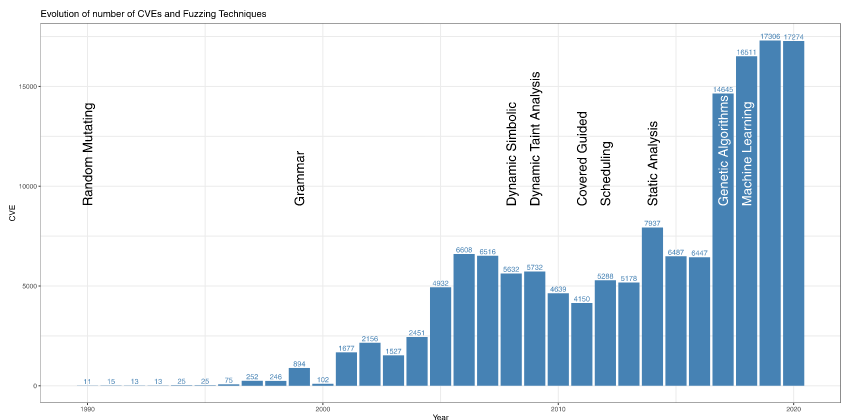
\includegraphics[width=\textwidth]{res/entwicklung_der_eingabestrategien}
    \caption{Eine Übersicht der Entwicklung von Eingabestrategien und deren Einfluss auf die Anzahl der neu aufgedeckten Schwachstellen
    über Zeit.
    Diese Abbildung wurde dem Paper von ~\citet{eceiza_fuzzing_2021} mit einverständnis nach der Creative Commons Attribution 4.0 Lizenz entnommen.}
    \label{fig:eingabestrategien}
\end{figure*}
Die Generierung von Eingabedaten ist ein zentraler Bestandteil des Fuzzings.
Die Qualität und Vielfalt der generierten Eingaben beeinflussen die Effektivität des Fuzzings.
Direkt verbunden mit der Entwicklung von Eingabegenerationsstrategien sind die Anzahl der neu aufgedeckten Schwachstellen (siehe Abb.\ ~\ref{fig:eingabestrategien}).
\subsection{Zufällige Mutation}\label{subsec:zufallige-mutation}
Die Random Mutation beinhaltet die Veränderung von Teilen einer Eingabe, um neue Testfälle für das
Fuzzing zu generieren.
Mutationsbasierte Fuzzer treffen dabei zwei entscheidende Entscheidungen: Wo soll die Mutation erfolgen und welchen neuen
Wert soll sie annehmen?
Häufige Techniken umfassen die Zufallsmodifikation von Bits, gezielte Bit-Flip-Operationen und Änderungen an Ganzzahlen.
Allerdings fehlt diesen Fuzzern das Bewusstsein für das erwartete Eingabeformat, was ihre Effektivität einschränken kann~\cite{saavedra_review_2019}.
\subsection{Regel- und Grammatikbasierte Mutation}\label{subsec:regelbasierte-muataion-und-grammatik}
Regel- und grammatikbasierte Mutationsansätze nutzen Eingabespezifikationen, um die Generierung neuer Eingaben gezielt
zu steuern.
Die Eingabesperifikationen können in Form von Grammatiken, regulären Ausdrücken oder anderen formalen Sprachen vorliegen,
welche der Anwender des Fuzzers zuvor selbst festlegen muss.
Diese Fuzzer erzielen eine bessere Codeabdeckung im Vergleich zu rein mutationsbasierten Fuzzern, da sie auf dem Wissen
über erwartete Eingabeformate basieren.
Allerdings erfordert die Entwicklung präziser Spezifikationen erheblichen Aufwand, was die Implementierung solcher Techniken
komplexer macht.
Diese Komplexität is besonders unter proprietären Softwarelösungen ohne verfügbaren Quellcode problematisch~\cite{eceiza_fuzzing_2021}.
\subsection{Dynamic Taint Analysis}\label{subsec:dynamic-taint-analysis}
Die Dynamic Taint Analyse verfolgt den Informationsfluss von Eingaben -- welche zur Laufzeit des Programms kontaminiert
werden -- zu sensiblen Operationen.
Sie ermöglicht die Erkennung von Schwachstellen, indem überwacht wird, wie Daten die Programmausführung beeinflussen.
Hierzu werden Speicherbereiche wie bspw.\ Register oder Speicherzellen markiert, um den Informationsfluss zu verfolgen.
Herausforderungen wie Overtainting und Undertainting können jedoch die Genauigkeit der Analyse beeinträchtigen, was zu
Fehlalarmen oder übersehenen Schwachstellen führt.
Overtainting tritt auf, wenn zu viele Daten als kontaminiert markiert werden, obwohl sie nicht kontaminiert wurden und
valide Eingaben darstellen und somit falschen Alarm schlagen.
Undertainting trifft zu, wenn kontaminierte Eingaben nicht als solche markiert werden~\cite{schwartz_all_2010}.
\subsection{Dynamic Symbolic execution}\label{subsec:dynamic-symbolic-execution}
Dynamic Symbolic Execution ermöglicht eine Sicherheitsanalyse, indem die Codeausführung überwacht und logische Formeln
erstellt werden, die die Ausführungspfade beschreiben.
Diese Technik hilft, Schwachstellen zu identifizieren, indem unterschiedliche Programmzustände erkundet werden.
Sie kann mit anderen Techniken wie der dynamischen Taint-Analyse kombiniert werden, um die Effektivität zu steigern.
Hier~\cite{schwartz_all_2010}
\subsection{Guided Covered}\label{subsec:guided-covered}
Techniken zur Guided Coverage nutzen Codepfade, um Strategien zur Eingabegenerierung zu
steuern.
Ziel ist es viele Programmpfade mit möglichst wenigen Eingaben zu traversieren.
Die Programmabdeckung wird dabei mithilfe von Instrumentierungstechniken, wie bspw.\ virtuellen Laufzeitumgebungen oder
Injektion eigener Instruktionen (Flags) in den Programmcode, gemessen~\cite{eceiza_fuzzing_2021}.
\subsection{Scheduling}\label{subsec:scheduling}
Das Input Scheduling ist eine Gray-box technik und kann in zwei phasen unterteilt werden:
\begin{enumerate}
    \item \textit{Explorationsphase}: In dieser Phase wird der Speicher teilweise markiert, um Eingabewerte im Speicher
    zu beobachten, wenn bestimmte Instruktionen, wie Vergleichsoperationen, ausgeführt werden.
    Diese Analyse des Speichers ermöglicht es, Eingabewerte mit Speicherzuständen zu verknüpfen (als Konfiguration bezeichnet)
    und fundierte Vermutungen darüber anzustellen, welche Werte ersetzt werden sollten~\cite{eceiza_fuzzing_2021}.
    \item \textit{Exploitationsphase}: In dieser Phase werden die generierten Eingaben teilweise kontaminiert und anhand des
    Feedbacks des SUT erraten, welche Werte ersetzt werden sollten.
    Die bereits gesammelten Daten werden zum Erraten neuer, potenziell schädlicher Werte verwendet~\cite{eceiza_fuzzing_2021}.
\end{enumerate}
\subsection{Statische Analyse}\label{subsec:statische-analyse}
Die statische Analyse untersucht den Code, ohne ihn auszuführen, und ermöglicht so die Identifikation potenzieller
Schwachstellen und Probleme in der Codequalität.
Diese Technik ergänzt dynamische Analyseansätze, da sie Einblicke in die Code-Struktur und mögliche Schwachstellen bietet,
die während der Ausführung nicht erkennbar sind~\cite{wang_systematic_2020}.
\subsection{Genetische Algorithmen}\label{subsec:genetische-algorithmen}
Diese Technik kann als Black-box-, Gray-box- oder White-box-Ansatz umgesetzt werden.
Sie nutzt ein suchbasiertes Optimierungsverfahren, das nach dem Prinzip der natürlichen Selektion arbeitet, um die
bestmöglichen Lösungen für komplexe Probleme zu finden.
Im Bereich des Fuzzings wird die Suche nach Schwachstellen als Optimierungsproblem betrachtet, wobei jede Kandidatenlösung
(Individuum) eine mögliche Fuzzing-Eingabe darstellt.
Die Tauglichkeit bewertet die Nähe zu einer Schwachstelle im SUT, basierend auf dynamischen und
statischen Informationen, wie z.B.\ strukturelle Komplexität~\cite{eceiza_fuzzing_2021}.
